\chapter{Detailed Report}\label{chapter:detailed_report}

\section{Tool description}

TODO:\newline
compare the 8 different tools used by your team. Which vulnerabilities can each
tool find? Which vulnerabilities can they not find?\newline
Tools generally find a large number of false positives. You must check if the results given to you by tools
are false positives or not. Write in the report what the percentage of false positives are for each tool and
for each type of vulnerability that the tool finds.

\subsection*{Web Testing Tools}

\subsubsection*{SSL Testing Shell script}
\begin{itemize}
	\item \textbf{Used by}\\ Mahmoud Naser
	\item \textbf{Used for}\\
	This tool was very useful in identifying SSL vulnerabilities and ciphers, it was a ready-to-use tool listed OWASP website, sample screen shots of the output are provided in figures \autoref{figure:bs_ssl_cipher}, \autoref{figure:bs_ssl_vuln}, \autoref{figure:gnb_ssl_cipher} and \autoref{figure:bs_ssl_vuln} 
	\item \textbf{Useful in}\\ \vulnref{OOTG-CRYPST-001}.
	It detected that both applications were vulnerable to POODLE and \bs was also vulnerable to Heartbleed.
\end{itemize}

\subsubsection*{devbug.co.uk}
\begin{itemize}
	\item \textbf{Used by}\\ Alexander Lill
	\item \textbf{Used for}\\
	DevBug is a basic PHP Static Code Analysis (SCA) tool written mostly in JavaScript. The idea behind DevBug is to make basic PHP Static Code Analysis accessible online, to raise security awareness and to integrate SCA into the development process. DevBug can be used to quickly test a page of PHP that you think may have some potential vulnerabilities, to run across a piece of code you have found on Google that you are unsure of or to directly write your own code in.
	
	This tool was used as an additional resource for Static Code Analysis reports.
	
	The website shows e.g. Cross-Site-Scripting and Command Injection vulnerabilities.
	\item \textbf{Useful in}\\ \vulnref{OTG-INPVAL-001} and \vulnref{OTG-INPVAL-002}
\end{itemize}

\subsubsection*{Kiuwan}
\begin{itemize}
	\item \textbf{Used by}\\ Alexander Lill
	\item \textbf{Used for}\\
	Kiuwan (see \url{https://www.kiuwan.com}) is a software as a service (SaaS) static program analysis multi-technology software for software analytics, quality and security measurement and management.
	
	This tool was used as a main source for possible vulnerabilities using Static Code Analysis.
	
	The tool shows defects in the categories "Maintainability", "Security", "Efficiency","Portability" and "Reliability" (see \autoref{figure:kiuwan}) as well as estimates for the effort to fix those issues. It can be connected with e.g. Github and automatically analyzes the code after every commit and shows metrics.
	\item \textbf{Useful in}\\ \vulnref{OTG-INPVAL-001} and \vulnref{OTG-INPVAL-002}
\end{itemize}

\begin{figure}[h!tbp]
	\centering
	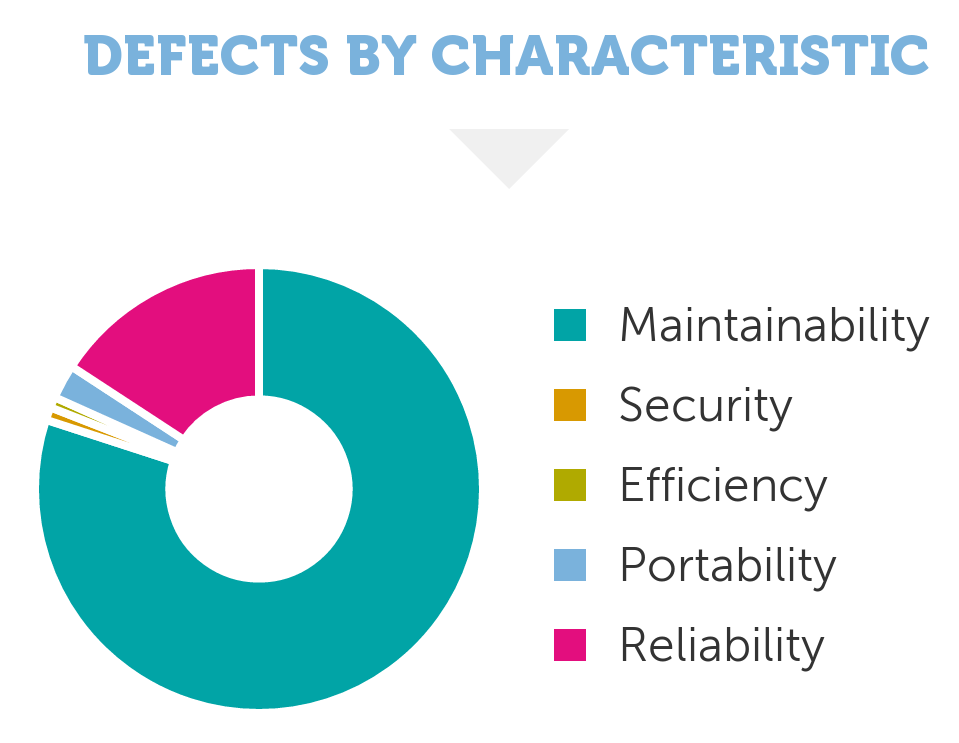
\includegraphics[width=0.5\textwidth]{figures/kiuwanResults}
	\caption{Example graph from Kiuwan}
	\label{figure:kiuwan}
\end{figure}

\subsubsection*{Advanced REST Client}
\begin{itemize}
	\item \textbf{Used by}\\ Alexander Lill, Lorenzo Donini
	\item \textbf{Used for}\\
	This tool provides a very useful interface to send a variety of HTTP requests and shows all the attributes of the responses and sent requests. It can be used to create specific requests including customized parameters as well as checking for resulting error codes / error messages and how long it took the web server to process the request.
	\item \textbf{Useful in}\\ \vulnref{OTG-ERR-002}, \vulnref{OTG-ERR-001}, \vulnref{OTG-SESS-005} and \vulnref{OTG-BUSLOGIC-004}
\end{itemize}

\subsubsection*{Cookie Inspector}
\begin{itemize}
	\item \textbf{Used by}\\ Alexander Lill
	\item \textbf{Used for}\\
	This tool provides the possibility to read, write and modify cookies. It also enables to examine the cookies which shows all their attributes. It was used to examine the cookies attributes and create customized cookies for testing and exploitation.
	\item \textbf{Useful in}\\ \vulnref{OTG-SESS-002}, \vulnref{OTG-SESS-005} and \vulnref{OTG-SESS-006}
\end{itemize}

\subsubsection*{RIPS}
\begin{itemize}
	\item \textbf{Used by}\\ Mahmoud Naser
	\item \textbf{Used for}\\ This tool was used to test PHP code on both \bs and \gnb

	\item \textbf{Useful in}\\ 	While most errors found using this tool were false positives, it did point out a few variables that were not immediately sanitized in the code in index.php for \bs but after further inspection variables were sanitized and checked at a later stage.
\end{itemize}

\subsubsection*{RATS}
\begin{itemize}
	\item \textbf{Used by}\\ Mahmoud Naser
	\item \textbf{Used for}\\ This tool was used to test PHP code on both \bs and \gnb.
	\item \textbf{Useful in}\\ This tool while useful in detecting SQL injection, unsanitized inputs etc, it did not provide much insight due to the quality of the used code .
\end{itemize}

\subsubsection*{Comparison}
TODO: Comparison Text


\subsection*{C and Java Testing Tools}

\subsubsection*{Java Decompiler}
\begin{itemize}
	\item \textbf{Used by}\\ Lorenzo Donini
	\item \textbf{Used for}\\ The Java decompiler standalone application was used to obtain the Java source code of the SCS application developed by \bs, given the compiled \texttt{.jar} file. Once decompiled, all the classes were exported and analyzed with separate tools. The Java decompiler was obtained from \texttt{http://jd.benow.ca/}.
	\item \textbf{Useful in}\\ No major vulnerabilities were found using this tool, but for a more in-depth description of how this tool was used, refer to \ref{chapter:reverse_engineering}.
\end{itemize}

\subsubsection*{FindBugs Intellij IDEA Plugin}
\begin{itemize}
	\item \textbf{Used by}\\ Lorenzo Donini
	\item \textbf{Used for}\\ This plugin for the Intellij IDEA Java IDE (software by JetBrains) was used to statically analyze the already decompiled Java source code of the whole SCS application developed by \bs. The tool returns a list of explicit vulnerabilities, bugs, dodgy code and more, with details about each entry and suggestions on how to fix them.
	\item \textbf{Useful in}\\ No major vulnerabilities were found using this tool, but for a more in-depth  description of how this tool was used, refer to \ref{chapter:reverse_engineering}.
\end{itemize}

\subsubsection*{IDA Pro - Free}
\begin{itemize}
	\item \textbf{Used by}\\ Lorenzo Donini, Florian Mauracher
	\item \textbf{Used for}\\ IDA Pro was used in order to reverse engineer the C parser binaries of the \bs{} application. The tool allowed us to interactively disassemble the compiled code and reverse engineer the whole parser starting from the assembly x86 instructions.\newline
	The main functionalities of IDA Pro that we used were the program-flow graph view, the strings view and the renaming of variables and locations with humand-readable logical names.
	\item \textbf{Useful in}\\ This tool didn't provide any direct insight on potential vulnerabilities, but allowed to retrieve the source code from the C parser binaries, needed for a further analysis. For a more in-depth description of the reverse engineering process, refer to \ref{chapter:reverse_engineering}.
\end{itemize}

\subsubsection*{variable\_mapper.py}
\begin{itemize}
	\item \textbf{Used by}\\ Lorenzo Donini
	\item \textbf{Used for}\\ We developed this script ourselves to aid us in the analysis of the assembly instructions of the C source code. 
	This tool works in conjunction with the IDA Pro software, allowing us to automatically generate a table of variable mappings, given the assembly instructions from IDA Pro in which memory locations on the stack are declared. These locations are usually mapped to specific variables in the source code, and finding out the size of each variable/pointer on the stack can provide useful information for the whole reverse engineering process.\newline
	This custom python script parses a txt file containing all declared stack variables and arguments, analyzes the size of each one by checking the memory location of consecutive variables and finally generates an Excel sheet in which these raw variables are mapped.\newline
	The source txt file looks like this:\newline
	\texttt{.text:08048AD1 var\_2E4         = dword ptr -2E4h \\
		.text:08048AD1 var\_2E0         = dword ptr -2E0h \\
		.text:08048AD1 var\_2D9         = byte ptr -2D9h \\
		.text:08048AD1 var\_2D8         = dword ptr -2D8h}\newline
	The script is located in our project repository under \texttt{/phase4/Team7/tools/variable\_mapper.py}, together with a README file and an Excel file \texttt{variables.xlsx} containing the generated variable mapping.
	
	\item \textbf{Useful in}\\ This tool was useful for speeding up the reverse engineering process of the C source code, since it allowed us to have a lookup table for all variables; it also helped us to figure out the types of each variable.
\end{itemize}

\subsubsection*{Radare2}

\subsubsection*{Comparison}
TODO: Comparison Text

\clearpage

TODO:\newline
describe identified vulnerabilities mentioning the following for each one
\begin{itemize}
	\item Observation: which part of the application is vulnerable and why?
	\item Discovery: how was this vulnerability discovered? Which tools were used and which steps were performed?
	\item Likelihood: what is the likelihood that this vulnerability is exploited? Which assumptions must hold and which skills must an attacker have?
	\item Impact: what is the potential impact of an exploit of this vulnerability? What could happen?
	\item Recommendation: how exactly would you fix this problem?
	\item Instantiate the CVSS v3.0 template for this particular vulnerability.
	\item Comparison with your own application: how and why is your app better/worse
\end{itemize}

NOTR: Each vulnerability should be described on a new page!\newline

\clearpage
%Sample tables
\vultable{\bs}{%
	Observation: which part of the application is vulnerable and why?
}{%
	Discovery: how was this vulnerability discovered? Which tools were used and which steps were performed?
}{%
	Likelihood: what is the likelihood that this vulnerability is exploited? Which assumptions must hold and which skills must an attacker have?
}{%
	Impact: what is the potential impact of an exploit of this vulnerability? What could happen?
}{%
	Recommendation: how exactly would you fix this problem?
}{%
	\na
	%\secure
	%\cvssBaseScorePretty{N}{H}{N}{R}{U}{H}{H}{N}
}
\vultable{\gnb}{%
	Observation: which part of the application is vulnerable and why?
}{%
	Discovery: how was this vulnerability discovered? Which tools were used and which steps were performed?
}{%
	Likelihood: what is the likelihood that this vulnerability is exploited? Which assumptions must hold and which skills must an attacker have?
}{%
	Impact: what is the potential impact of an exploit of this vulnerability? What could happen?
}{%
	Recommendation: how exactly would you fix this problem?
}{%
	\na
	%\secure
	%\cvssBaseScorePretty{N}{H}{N}{R}{U}{H}{H}{N}
}
Comparison with your own application: how and why is your app better/worse
\clearpage

\section{Configuration and Deploy Management Testing}
\simpleVulntitle{OTG-CONFIG-003}{Test File Extensions Handling for Sensitive Information}
\vultable{\bs}{%
	We discovered that it is possible to access some files and directories which should not be accessible to the user/attacker. Specifically, we were able to get a hold of the private key used by the server for SSL encryption, the MySQL dump file and other data that should not be accessible from the network and, even less, to attackers.
}{%
	We managed to directly download several files containing sensitive information directly, as well as access some unprotected content:
	\begin{itemize}
		\item \texttt{http://[HOST]/app/HTTPS/hostonly.key}
		\item \texttt{http://[HOST]/adminer}
		\item \texttt{http://[HOST]/dump.sql}
		\item \texttt{http://[HOST]/Smart-Card-Simulator/src/scs/Main.java}, as well as all other Java sources.
	\end{itemize}
	Also many other README and temporary files are directly accessible.
}{%
	Since directory listing is disabled inside the /api and /app subfolders of the application, most of the mentioned files can be accessed only via brute-force attacks, and even then it would prove very difficult to guess the name of the directory and filename correctly. During white-box testing, this was not an issue, but in reality, finding out this weakness would require much time (low likelihood). Other names of files, however, contained in the root folder (directory listing here is not disabled), like dump.sql can be easily guessed.
}{%
	Although an attacker cannot directly compromise the integrity and availability of the server, it is possible to access some very important content of the application. In particular, getting a hold of \texttt{hostonly.key} allows to start MITM attacks on any victim, since the file contains the private key of the server used for SSL encryption.
}{%
	Relocate the .htaccess files (or the root of the web application) and place more strict rules for file/directory access, since these are too loose.
}{%
	\cvssBaseScorePretty{N}{L}{N}{N}{U}{H}{N}{N}
}
\vultable{\gnb}{%
	The Apache server is configured globally for the whole application, disabling directory listing but allowing direct access to all files inside the web folder. This folder mainly contains PHP, Javascript, HTML, CSS and media files (images). Among these, no sensitive information can be leaked. We found, however, that the upload folder contents are potentially accessible. So, if an attacker could brute-force the name of an uploaded file (which is entirely random) before it gets deleted by the server, he could read the contents.
}{%
	We accurately analyzed the Apache configuration on the \gnb{} system and then tested different cases manually.
}{%
	For an attacker to be successful, he would not only have to guess the name of a file correctly, but also request it in the time window in which the file gets parsed by the C parser, before it is deleted. This time window is very slim, making the likelihood of this attack very low.
}{%
	Assuming such an attack is successful, an attacker could read the contents of a batch transaction file uploaded by a user. The confidentiality implications are not very high, considering the file doesn't contain any sensitive information such as passwords; however, since the \gnb{} application renames the files with the SessionID of the user who uploaded the file, having guessed the name of a file gives information about the SessionID of the user, allowing session hijacking.\newline
	Given that only client sessions could be hijacked this way, the implications affect only confidentiality, and not integrity or availability, since no sensitive information is leaked whatsoever.
}{%
	Disable some file extensions for the web application in the Apache configuration, such as txt.
}{%
	\cvssBaseScorePretty{N}{H}{N}{R}{U}{L}{N}{N}
}

\vulntitle{OTG-CONFIG-006}{Test HTTP Methods}
\vultable{\bs}{%
	We observed that the GET, POST, HEAD and OPTIONS methods are allowed over HTTPS. The methods PUT, DELETE and TRACE are not allowed, while other methods like COPY and MOVE are not implemented at all.
}{%
	This discovery was made by testing the available methods with the HTTPS client integrated in openssl. \newline (eg. \texttt{openssl s\_client -connect HOST:443})
}{%
	\na
}{%
	\na
}{%
	\na
}{%
	\secure
}
\vultable{\gnb}{%
	We observed that the GET, POST, HEAD and OPTIONS methods are allowed over HTTPS. The methods PUT, DELETE and TRACE are not allowed, while other methods like COPY and MOVE are not implemented at all.
}{%
	This discovery was made by testing the available methods with the HTTPS client integrated in openssl. \newline (eg. \texttt{openssl s\_client -connect HOST:443})
}{%
	\na
}{%
	\na
}{%
	\na
}{%
	\secure
}

\vulntitle{OTG-CONFIG-007}{Test HTTP Strict Transport Security}
\vultable{\bs}{%
	Although HTTPS is enabled on port 443, access to the page without using HTTPS is still possible, by simply accessing the server on port 80. However, since this was left on purpose by the developers for testing purposes, we decided not to treat this as a vulnerability (no CVSS score is given).
}{%
	This information was given to us directly by the Team that developed the Bank System application. We also proved this by simply trying to access the application on port 80: this way we had normal access to the application, although without any transport security.
}{%
	Since we are not considering this as a vulnerability, we won't analyze it in depth.
}{%
	The implications of lack of an encrypted connection were already analysed in phase 2. Since we are not considering this as a vulnerability anyway, we won't analyze its implications.
}{%
	Redirect any requests from port 80 to port 443. This is highly recommended before the application goes live.
}{%
	\secure
}
\vultable{\gnb}{%
	This vulnerability was fixed in phase 3 and the application is only allowing communication between the client and the server via HTTPS.
}{%
	We discovered this by simply testing to access both ports 80 and 443 on the webserver, which only allowed us to connect to the latter. A connection on port 80 was refused by the server. We also enforced this theory by checking it with nmap, getting the same result.
}{%
	\na
}{%
	\na
}{%
	\na
}{%
	\secure
}


\vulntitle{OTG-CONFIG-008}{Test RIA cross domain policy}
\vultable{\bs}{%
	Access to crossdomain.xml and clientaccesspolicy.xml was tested.
}{%
Access to crossdomain.xml and clientaccesspolicy.xml files were tested on all available directories as well as root directory and could not gain access to any of the following directories:

\begin{itemize}
	\setlength\itemsep{0pt}
	\item .
	\item app
	\item font
	\item pdfs
	\item src
	\item src/Api
	\item src/Api/Model
	\item tests
	\item tests/Test
	\item tests/Test/Functional
	\item tests/Test/Unit
	\item config
	\item parser
\end{itemize}	
}{%
\na
}{%
\na
}{%
\na
}{%
\secure
}
\vultable{\gnb}{%
	\same
}{%
Access to crossdomain.xml and clientaccesspolicy.xml files were tested on all available directories as well as root directory and could not gain access to any of the following directories:

\begin{itemize}  
	\setlength\itemsep{0pt}
	\item .
	\item ./project
	\item ./project/holder
	\item ./project/media
	\item ./project/lib
	\item ./project/templates
	\item ./project/js
	\item ./project/models
	\item ./project/accounts
	\item ./project/pwreset
	\item ./project/uploads
	\item ./project/client
	\item ./project/style
	\item ./project/registration
	\item ./project/employee
\end{itemize}	

}{%
\na
}{%
\na
}{%
\na
}{%
\secure
}

\clearpage
\section{Identity Management Testing}
\simpleVulntitle{OTG-IDENT-001}{Test Role Definitions}
\vultable{\bs}{%
	The role definitions are implemented as specified in their report for phase 2 and are secure.
}{%
	Manual testing and checking the contraints in the source code, e.g. \texttt{api/index.php}
}{%
	\na
}{%
	\na
}{%
	\na
}{%
	\secure
}
\vultable{\gnb}{%
	\same
}{%
	Manual testing and checking the contraints in the source code, e.g. \texttt{db.php}
}{%
	\na
}{%
	\na
}{%
	\na
}{%
	\secure
}



\vulntitle{OTG-IDENT-002}{Test User Registration Process}
\vultable{\bs}{%
	The registration process is set up for anyone to register, the process then awaits human interaction for the approval stage, this will serve an extra step of verification. Mail addresses have to be unique and can not be used by multiple users.
	
	Identities are not verified nor checked at this stage due to application limitations.
	
	No CAPTCHA or similar tests available to test if users are robots or human.
}{%
	Manual testing and checking the source code if duplicate mail addresses are possible. Here the database prevents the entry of a duplicate mail address, while the front end shows "Registration successful. Waiting for approval. You will be notified to email." even if the mail address was already in the dabase and the new account not successfully created.
}{%
	High. It is easy to create a lot of new users as long as a syntactically valid mail address is provided.
}{%
	Medium. A lot of new users could lead to performance or availability problems in the database. These registered users can not be used on the website as long as they are not approved, though.
}{%
	The introduction of CAPTCHAs, any other check for human users or some invitation mechanism might solve this issue.
}{%
	\cvssBaseScorePretty{N}{L}{N}{N}{U}{N}{N}{L}
}
\vultable{\gnb}{%
	\same
}{%
	Manual testing and checking the source code if duplicate mail addresses are possible. Here the database prevents the entry of a duplicate mail address and shows a message upon registration if the mail address was already used.
}{%
	\na
}{%
	\na
}{%
	\na
}{%
	\cvssBaseScorePretty{N}{L}{N}{N}{U}{N}{N}{L}
}

\vulntitle{OTG-IDENT-003}{Test Account Provisioning Process}
\vultable{\bs}{%
	Provisioning clients is an easy process with no effective mechanisms
to verify or vet clients besides a manual approval process, provisioning employees is set up in a similar matter.
Vulnerabilities with creating the client account have been discussed
in the previous section \vulnref{OTG-IDENT-002}, the same applies to creating
employee accounts, so a potential DOS attack is possible by creating
robot accounts.
}{%
	This was found through following the given process for creating
accounts.
}{%
	High. It is easy to create a lot of new users as long as a syntactically valid mail address is provided.
}{%
	Medium. A lot of new users could lead to performance or availability problems in the database. These registered users can not be used on the website as long as they are not approved, though.
}{%
	The introduction of CAPTCHAs, any other check for human users or some invitation mechanism might solve this issue.
}{%
	\cvssBaseScorePretty{N}{L}{N}{N}{U}{N}{N}{L}
}
\vultable{\gnb}{%
	\same
}{%
	\same
}{%
	\same
}{%
	\same
}{%
	\same
}{%
	\cvssBaseScorePretty{N}{L}{N}{N}{U}{N}{N}{L}
}

\vulntitle{OTG-IDENT-004}{Testing for Account Enumeration and Guessable User Account}
\vultable{\bs}{%
	The user account names are the users mail addresses and therefore not easily guessable. The \bs{} is vulnerable for Account Enumeration: Logins with an associated mail address and a wrong password lead to the message "Incorrect data. Wrong user or password. You have X tries more.", while a login with an unassociated mail address and any password leads to the message "Incorrect data. Wrong user or password".
}{%
	This was discovered manually in the source code (file \texttt{api/index.php} lines 178-180 and 214-245) and confirmed by manual testing.
}{%
	The use of this vulnerability is very likely as this is a very easy way to get to know valid user accounts. Also see \vulnref{OTG-BUSLOGIC-004}.
}{%
	This vulnerability has a low impact as the only information that can be obtained is the email of a user, which doesn't provide any information about the password or other sensitive information.
}{%
	We recommend to always show the same error message, even though the user does not see how many tries he still has left.
}{%
	\cvssBaseScorePretty{N}{L}{N}{N}{U}{L}{N}{N}
}
\vultable{\gnb}{%
	The \gnb{} application is always showing the same error message and is thus not vulnerable. We do also use the users mail address as user account names which makes them not easily guessable.
}{%
	\na
}{%
	\na
}{%
	\na
}{%
	\na
}{%
	\secure
}

\vulntitle{OTG-IDENT-005}{Testing for Weak or unenforced username policy}
\vultable{\bs}{%
	Username has to be in valid email address format.
}{%
	This was found through trial and error and checking the according files (e.g. \texttt{index.php}, line 483).
}{%
	\na
}{%
	\na
}{%
	\na
}{%
	\secure
}
\vultable{\gnb}{%
	\same
}{%
	This was found through trial and error and checking the according files (e.g. \texttt{js/registration.js} line 81, \texttt{registration/registration\_request.php} line 29).
}{%
	\same
}{%
	\same
}{%
	\same
}{%
	\secure
}

\clearpage
\section{Authentication Testing}
\simpleVulntitle{OTG-AUTHN-001}{Testing for Credentials Transported over an Encrypted Channel}
\vultable{\bs}{%
	All request to the site are done over an encrypted HTTPS connection. No unencrypted messages were observed.
	% HTTP still enabled
}{%
	After capturing the traffic during login with wireshark, it was verified that all requests made were encrypted.
}{%
	\na
}{%
	\na
}{%
	\na
}{%
	\secure
	%\cvssBaseScorePretty{N}{H}{N}{R}{U}{H}{H}{N}
}
\vultable{\gnb}{%
	All request to the site are done over an encrypted HTTPS connection. No unencrypted messages were observed.
	% HTTP port disabled
}{%
	After capturing the traffic during login with wireshark, it was verified that all requests made were encrypted.
}{%
	\na
}{%
	\na
}{%
	\na
}{%
	\secure
}

\vulntitle{OTG-AUTHN-002}{Testing for default credentials}
\vultable{\bs}{%
	The developers left a temporary administrator test account with weak credentials. It is likely that this was done specifically for testing purposes, but we decided to treat this as a vulnerability anyway, since this should be avoided when the application goes live.\newline
	This flaw aside, no other accounts with weak credentials were found; also passwords are not automatically generated for users and the password policy is strict, not allowing weak passwords or empty fields for that matter.
}{%
	The default credentials left for testing purposes were:\newline
	\texttt{user: test4@test.org pass: test}\newline
	These were given to us directly by the developers. To prove our point, we also searched through the Rocktyou.txt password list (found at \texttt{https://wiki.skullsecurity.org/index.php?title=Passwords} and proved that 'test' is a very weak password.
}{%
	The likelihood of cracking the password is high. Brute-forcing the username may require some more effort, but since the application returns different error codes depending whether the inserted username or password were wrong, an attacker can easily try out any possible username.
}{%
	In this particular case the implications are severe, since a successful attack would grant an attacker admin rights, with consequent full access to the application.
}{%
	It is highly recommended to change the default credentials of the application admin before deploying the application.
}{%
	\cvssBaseScorePretty{N}{L}{L}{N}{U}{L}{N}{H}
}

\vultable{\gnb}{%
	The same observations made for Bank System apply. Furthermore, no weak default credentials were left at all (not even for testing purposes).
}{%
	\na
}{%
	\na
}{%
	\na
}{%
	\na
}{%
	\secure
}


\vulntitle{OTG-AUTHN-003}{Testing for Weak lock out mechanism}
\vultable{\bs}{%
	The lockout mechanism was implemented in phase 3 on all systems as part of the requirements. 
}{%
Multiple incorrect logins were attempted, until the account was locked for 15 minutes after 6 incorrect attempts.
}{%
\na
}{%
\na
}{%
\na
}{%
\secure
}
\vultable{\gnb}{%
	\same
}{%
Multiple incorrect logins were attempted, until the account was locked after 5 incorrect attempts, the account can only be unlocked manually by an employee account.

}{%
\na
}{%
\na
}{%
\na
}{%
\secure
}

\vulntitle{OTG-AUTHN-004}{Testing for bypassing authentication schema}
\vultable{\bs}{%
	No way to bypass the authentication schema was discovered. All internal
	pages properly redirect to the login page.
}{%
	A controller is responsible for routing the requests, after looking at it's
	source it could be verified, that no internal pages are accessible without
	authentication.
}{%
	\na
}{%
	\na
}{%
	\na
}{%
	\secure
}
\vultable{\gnb}{%
	No way to bypass the authentication schema was discovered. All internal
	pages properly redirect to the login page.
}{%
	After inspecting the code, all php sites only meant for an authenticated
	user appear to check for a valid user session before further processing the
	request.
}{%
	\na
}{%
	\na
}{%
	\na
}{%
	\secure
}


\vulntitle{OTG-AUTHN-005}{Test remember password functionality}
\vultable{\bs}{%
	Password is only transmitted during the login phase, and stored in a secure
	way server side.
}{%
	A strong hash function is used in combination with a salt to store the
	password in the database: \newline
	\texttt{hash('sha256', \$plainpassword.\$salt);}
}{%
	\na
}{%
	\na
}{%
	\na
}{%
	\secure
}
\vultable{\gnb}{%
}{%
	Password is only transmitted during the login phase, and stored in a secure
	way server side.
}{%
	A strong hash function is used in combination with a salt to store the
	password in the database: \newline
	\texttt{hash('sha512', \$this->MAGIC . \$password . \$salt);} \newline
	MAGIC is an additional token hardcoded in the php code and \texttt{sha512}
	offers additional entropy compared to \texttt{sha256}, so the \gnb{}
	application is slightly more secure here.
}{%
	\na
}{%
	\na
}{%
	\secure
}

\vulntitle{OTG-AUTHN-006}{Testing for Browser cache weakness}
\vultable{\bs}{%
	We observed that no Browser cache weaknesses could be exploited for this web application. This statement only holds when HTTPS is enforced (see \vulnref{OTG-CONFIG-007}). It is important to stress though, that the Bank System application does not explicitly avoid cache weaknesses, as can be seen in any intercepted server response. This is not a problem, however, since the used Framework dynamically loads the sensitive information of the page using asynchronous Ajax requests, which are not cached by the browser.
}{%
	Browser history was tested manually, showing no issues.\newline 
	The browser cache was tested using the CacheViewer2 addon for Firefox: this showed us that server responses are actually cached by the browser, but these are encrypted as long as HTTPS is used. Also, given that Bank System dynamically loads pages, we only managed to restore some pages from the cache.
}{%
	\na
}{%
	\na
}{%
	Although the application didn't show evident browser cache weaknesses, it is still recommended to set some additional cache-control: no-cache, no-store, must-revalidate.
}{%
	\secure
}

\vultable{\gnb}{%
	The \gnb{} application enforces cache invalidation, preventing the browser from storing any sensible information other that stylesheets and javascript files locally. Browser history also couldn't be exploited, since the application delivers the pages over HTTPS.
}{%
	Browser history was tested manually, showing no issues. Browser cache was tested using the CacheViewer2 addon for Firefox. We also analyzed some responses from the server, only to see that the application sets the following flags:\newline
	\texttt{Cache-Control: private, must-revalidate}
}{%
	\na
}{%
	\na
}{%
	\na
}{%
	\secure
}
\vulntitle{OTG-AUTHN-007}{Testing for Weak password policy}
\vultable{\bs}{%
	The weak password policy was rectified as a requirement in phase 3 on all systems. 
}{%
Registration attempts were made with weak passwords, all attempts failed.
}{%
\na
}{%
\na
}{%
\na
}{%
\secure
}
\vultable{\gnb}{%
	\same
}{%
	\same
}{%
\na
}{%
\na
}{%
\na
}{%
\secure
}
\vulntitle{OTG-AUTHN-008}{Testing for Weak security question/answer}
\vultable{\bs}{%
	\notImp
}{%
	\na
}{%
	\na
}{%
	\na
}{%
	\na
}{%
	\na
}
\vultable{\gnb}{%
	\notImp
}{%
	\na
}{%
	\na
}{%
	\na
}{%
	\na
}{%
	\na
}

\vulntitle{OTG-AUTHN-009}{Testing for weak password change or reset functionalities}
\vultable{\bs}{%
	\textbf{Password change:} \newline
		A logged in user is able to change his password by supplying his
		current password. This is considered safe. \newline
	\textbf{Password reset:} \newline
		A password reset can be requested by an unauthenticated user, by
		supplying the email address of the account on the web page.
		An email with a password reset link is sent to the specified address,
		where the password can be reset without further authentication.
		This enables an attacker with control over the email address to take
		over the account.
}{%
	The change password functions were tested manually.
}{%
	Unlikely. Attacker needs control over the email account of the victim.
}{%
	High for a single account. The attacker gains full control over the victims account.
}{%
	Require an additional secret to reset the password and identify the user.
	This could be a security question or the PIN. (As long as its clearly
	stated that the user needs to store it safely)
}{%
	\cvssBaseScorePretty{N}{H}{L}{N}{U}{L}{L}{L}
}
\vultable{\gnb}{%
	\textbf{Password change:} \newline
		\notImp \newline
	\textbf{Password reset:} \newline
		A password reset can be requested by an unauthenticated user, by
		supplying the email address of the account on the web page.
		An email with a password reset link is sent to the specified address,
		where the password can be reset by specifying the account PIN.
		This second factor prevents an attacker with control over the email
		address to take over the account.
}{%
	The password reset function was tested manually.
}{%
	\na
}{%
	\na
}{%
	\na
}{%
	\secure
}

\vulntitle{OTG-AUTHN-010}{Testing for Weaker authentication in alternative channel}
\vultable{\bs}{%
	The application does not provide alternative channels for authentication. The separate Smart Card Simulator Java application does not communicate with the server directly and does not perform any authentication for the user, hence this vulnerability is not applicable.
}{%
	\na
}{%
	\na
}{%
	\na
}{%
	\na
}{%
	\na
}
\vultable{\gnb}{%
	The same observation made for the \bs application applies.
}{%
	\na
}{%
	\na
}{%
	\na
}{%
	\na
}{%
	\na
}

\clearpage
\section{Authorization Testing}
\simpleVulntitle{OTG-AUTHZ-001}{Testing Directory traversal/file include}
\vultable{\bs}{%
	This was done through blackbox testing using ZED proxy tool and a variation of the commands bellow :
	
	\begin{itemize}  
		\item egrep -r \lq(include|require|fopen|readfile)\rq .
		\item egrep -r \lq\$\_(POST|GET|FILE)\rq . 
	\end{itemize}
}{%
No vulnerabilities were found for this application.
}{%
\na
}{%
\na
}{%
\na
}{%
\secure
}
\vultable{\gnb}{%
	This was fixed in phase 3 as part of the requirements.
}{%
\same
}{%
\na
}{%
\na
}{%
\na
}{%
\secure
}
\vulntitle{OTG-AUTHZ-002}{Testing for bypassing authorization schema}
\vultable{\bs}{%
	No vulnerabilities in this area were found for the \bs{} application.
}{%
	This was observed by checking all necessary functions in the file \texttt{api/index.php} which does all the checks if a request is valid or not and some manual trial and error testing.
}{%
	\na
}{%
	\na
}{%
	\na
}{%
	\secure
}
\vultable{\gnb}{%
	No vulnerabilities in this area were found for the \gnb{} application.
}{%
	This was observed by checking all necessary functions in the according files and some manual trial and error testing.
}{%
	\na
}{%
	\na
}{%
	\na
}{%
	\secure
}

\vulntitle{OTG-AUTHZ-003}{Testing for Privilege Escalation}
\vultable{\bs}{%
	No vectors for privilege escalation could be identified in the \bs{}
	application.
}{%
	After inspecting the source of the controller responsible for routing the
	requests, it appears that all pages requiring elevated permissions
	correctly verify that these elevated permissions are present.
}{%
	\na
}{%
	\na
}{%
	\na
}{%
	\secure
}
\vultable{\gnb}{%
	No vectors for privilege escalation could be identified in the \gnb{}
	application.
}{%
	After inspecting the code, all php sites only meant for users with elevated
	permission appear to check for these permissions before further processing
	the request.
}{%
	\na
}{%
	\na
}{%
	\na
}{%
	\secure
}

\vulntitle{OTG-AUTHZ-004}{Testing for Insecure Direct Object References}
\vultable{\bs}{%
	All calls which involve retrieving sensitive information from the server are done via REST APIs. We analyzed all callback functions (contained inside the \texttt{/api/index.php} file) and tested the APIs manually, providing unexpected parameters. Doing this we did not manage to find any insecure direct object reference, since the server always checks whether the user issuing a request is allowed to perform a certain operation, preventing a malicious attacker to bypass the authorization schema. 
}{%
	We used the Advanced REST Client extension for Chrome in order to test the available APIs (e.g. \texttt{/api/getHistory} and \texttt{/api/userinfodetails}).
}{%
	\na
}{%
	\na
}{%
	\na
}{%
	\secure
}
\vultable{\gnb}{%
	The application performs thorough checks on every page on which application-specific functionalities are called (for example lines 7-22 inside the \texttt{/gnb/project/account/download\_transactions.php} file). These checks prevent users with to access data they're not allowed to access. We did not manage to find any insecure direct object reference this while analyzing the \gnb application.
}{%
	We used static PHP code analysis and also checked all server-side functionalities manually.
}{%
	\na
}{%
	\na
}{%
	\na
}{%
	\secure
}

\clearpage
\section{Session Management Testing}
\simpleVulntitle{OTG-SESS-001}{Testing for Bypassing Session Management Schema}
\vultable{\bs}{%
	This was done by checking the Session ID, Token Length, Session time-out mechanism and HTTPS
}{%
No vulnerabilities was found for this application.
}{%
\na
}{%
\na
}{%
\na
}{%
\secure
}
\vultable{\gnb}{%
	This was fixed in phase 3 as part of the requirements.
}{%
\same
}{%
\na
}{%
\na
}{%
\na
}{%
\secure
}

\vulntitle{OTG-SESS-002}{Testing for Cookies attributes}

\vultable{\bs}{%
	We observed that the \bs{} application is not setting all possible cookie attributes, see \autoref{table:cookieattributes}.
}{%
	This was discovered using manual examination of the cookies and additionally by checking the source code for cookie settings.
}{%
	The likelihood is quite high for the exploitation of the missing "HTTP only" and "secure" attributes. The missing "secure" attribute could be related to \vulnref{OTG-CONFIG-007}.
}{%
	This could have a quite big impact as Cookies could be transferred over an insecure connection. Additionally cookies can be read using Javascript e.g. by XSS vulnerabilities.
}{%
	We recommend to set the missing cookie attributes accordingly.
}{%
	\cvssBaseScorePretty{N}{L}{N}{R}{U}{L}{L}{N}
}

\vultable{\gnb}{%
	The \gnb{} application is setting all necessary and/or useful cookie attributes, see \autoref{table:cookieattributes}.
}{%
	\same
}{%
	\na
}{%
	\na
}{%
	\na
}{%
	\secure
}

\begin{table}
\centering
\begin{tabular}{| l | p{3cm} | p{3cm} |}
Attribute & 	\bs{} & \gnb{} \\
\toprule
Session & 		yes	& yes \\
\midrule
Host only &		yes	& yes \\
\midrule
HTTP only &		no	& yes \\
\midrule
Secure &		no	& yes \\
\midrule
Expiry date &	\multicolumn{2}{c|}{Not necessary because of "session" attribute} \\
\bottomrule

\end{tabular}
\caption{Cookies attributes}
\label{table:cookieattributes}
\end{table}

\vulntitle{OTG-SESS-003}{Testing for Session Fixation}
\vultable{\bs}{%
	A new session is generated after the user successfully logs in.
}{%
	This was tested manually and verified by inspecting the code responsible.
}{%
	\na
}{%
	\na
}{%
	\na
}{%
	\secure
}
\vultable{\gnb}{%
	A new session is generated after the user successfully logs in.
}{%
	This was tested manually and verified by inspecting the code responsible.
}{%
	\na
}{%
	\na
}{%
	\na
}{%
	\secure
}


\vulntitle{OTG-SESS-004}{Testing for Exposed Session Variables}
\vultable{\bs}{%
	We discovered that the only session variable used during the lifetime of the application is the SessionID, which is always exchanged between client and server using a Cookie. Although this cookie is not secure, this information is always transferred over an encrypted channel, not allowing MITM attacks.
}{%
	We tried capturing packets with Wireshark, in order to prove that the session ID is not visible by simply inspecting the encrypted packets.
}{%
	\na
}{%
	\na
}{%
	\na
}{%
	\secure
}
\vultable{\gnb}{%
	Similar to the case of the \bs{} application, the only session variable is the SessionID, which is transferred between client and server over an encrypted channel, not allowing MITM attacks.
}{%
	\same
}{%
	\na
}{%
	\na
}{%
	\na
}{%
	\secure
}

\vulntitle{OTG-SESS-005}{Testing for Cross Site Request Forgery}
\vultable{\bs}{%
	We observed a serious vulnerability in the Cross Site Request Forgery mechanism of the \bs{} application. The application only compares the client-side XSRF token sent in the cookie with the client-side token sent in the header of the request. That means that this token is useless if the one in the cookie as well as the one in the header are changed simultaneously on the client. Tokens are not stored server-side.
}{%
	We checked the source code for measures against CSRF and found the not properly working mechanism (see \texttt{api/asset.php} lines 48-63). We confirmed this vulnerability with manual testing and the tools "Advanced REST Client" and "Cookie inspector".
}{%
	Medium. It is quite likely that this vulnerability is quite easy to exploit.
}{%
	Medium. Any request sent to the \bs{} application website can be easily forged via Cross Site Scripting (also notice that the cookies are not secured against JavaScript manipulation, \vulnref{OTG-SESS-002}), but neither transactions nor password change requests can be executed as either a TAN or the current password is needed for that.
}{%
	We recommend to store the token value on the server instead and check the sent token against this one.
}{%
	\cvssBaseScorePretty{N}{H}{N}{R}{U}{L}{L}{N}
}
\vultable{\gnb}{%
	No Cross Site Request Forgery vulnerability was observed in the \gnb{} application.
}{%
	We checked the source code (e.g. see \texttt{accounts/new\_transaction.php} lines 17-23) for the CSRF algorithm and also observed a client-server session using the Chrome Developer Tools.
}{%
	\na
}{%
	\na
}{%
	\na
}{%
	\secure
}

\vulntitle{OTG-SESS-006}{Testing for logout functionality}
\vultable{\bs}{%
	We observed that the logout can be easily circumvented by just re-creating the old cookies with the same values before the logout. That means that we can easily undo the logout by just adding a cookie locally.
}{%
	We discovered this by manually looking through the source code and confirmed this by manual testing. \autoref{lst:logoutbug} shows the bug that makes this exploit possible. The variable \texttt{\$UserId} in line 15 is not defined in this context. leading to an SQL \texttt{UPDATE} statement with the following invalid \texttt{WHERE} clause: \texttt{where UserId='';}.
}{%
	It is very likely that this vulnerability will be exploited as cookies can be stolen quite easy (see \vulnref{OTG-SESS-002}) and this removes the timing aspect of stealing a given session. Logging out from the users session does not prevent any further attacks for this session.
}{%
	The potential impact of this vulnerability is high as this makes stealing a user's session much easier. An attacker only needs to get access to the users PHPSESSID or the not completely secure cookie.
}{%
	This issue can be easily resolved by using \texttt{\$user->UserId} instead if the undefined \texttt{\$UserId}.
}{%
	\cvssBaseScorePretty{N}{H}{N}{R}{U}{L}{L}{N}
}

\begin{minipage}{\linewidth}
\begin{lstlisting}[language=PHP, label={lst:logoutbug}, numbers=left, caption=Logout Bug]
    $app->get('/logout', function() use ($app, $db, $queries) {
        csrf_check();
        $user = getCurrentUserInfo();
        session_start();
        if (isset($_COOKIE['PHPSESSID'])) {
            setcookie('PHPSESSID', '', time() - 3600, '/');
        }
        if (isset($_COOKIE['XSRF-TOKEN'])) {
            setcookie('XSRF-TOKEN', '', time() - 3600, '/');
        }
        session_unset();   // Remove the $_SESSION variable information.
        session_destroy();// Remove the server-side session information.
        $query = $queries["updateSessionId"]();
        $statement = getStatement($query);
        $statement->bind_param('si', $sessionId, $UserId);
        $sessionId=NULL;
        $statement->execute();
        $statement->store_result();
    });
\end{lstlisting}
\end{minipage}

\vultable{\gnb}{%
	No vulnerabilities in the logout mechanism have been found in the \gnb{} application.
}{%
	\same
}{%
	\na
}{%
	\na
}{%
	\na
}{%
	\na
}

\vulntitle{OTG-SESS-007}{Test Session Timeout}
\vultable{\bs}{%
	A session timeout occurs after 20 minutes.
}{%
	The timeout found in the code was verified manually. After the timeout has
	occured, all furhter requests are denied.
}{%
	\na
}{%
	\na
}{%
	\na
}{%
	\secure
}

\vultable{\gnb}{%
	A session timeout occurs after approximately 24 minutes.
}{%
	The timeout is implemented by configuring the
	\texttt{session.gc\_maxlifetime} value.
	This does not appear to be the most reliable approach according to the
	documentation, but was confirmed working in practice.
}{%
	\na
}{%
	\na
}{%
	Implement a more reliable way for the session timeout.
}{%
	\secure
}


\vulntitle{OTG-SESS-008}{Testing for Session puzzling}
\vultable{\bs}{%
	While analyzing the source code, we found out that the SessionID is generated entirely randomly, using the PHP APIs (this can be seen inside the login callback function contained in \texttt{/api/index.php}). It is also used only for session tracking purposes, therefore no session puzzling vulnerability can occur.
}{%
	We manually analyzed the PHP source code of the target application.
}{%
	\na
}{%
	\na
}{%
	\na
}{%
	\secure
}
\vultable{\gnb}{%
	The \gnb{} application generates the SessionID entirely randomly and uses it for session tracking purposes as well as for replacing the names of the batch files. This, however, isn't a vulnerability, since the transaction batch files cannot be accessed through the network, once uploaded, and they are removed from the system as soon as the transaction has been executed.
}{%
	We manually analyzed the PHP source code of the target application.
}{%
	\na
}{%
	\na
}{%
	\na
}{%
	\secure
}

\clearpage
\section{Data Validation Testing}
\simpleVulntitle{OTG-INPVAL-001}{Testing for Reflected Cross Site Scripting}
\vultable{\bs}{%
	No Reflected Cross Site Scripting vulnerabilities have been found in the \bs{} application. There is only one place where user input is directly echoed onto a website, but this happens in the API (see \texttt{api/index.php} line 142) and is thus not visible.
}{%
	This was discovered by checking the results of RIPS (which only showed false positives), the results of \url{http://devbug.co.uk} and manually testing a few functionalities.
}{%
	\na
}{%
	\na
}{%
	\na
}{%
	\secure
}

\vultable{\gnb}{%
	No Reflected Cross Site Scripting vulnerabilities have been found in the \bs{} application. The only vulnerable page (\texttt{accounts/verify\_transaction.php}) uses proper sanitization to prevent Reflected Cross Site Scripting.
}{%
	This was discovered by checking the results of RIPS (which only showed false positives), the results of \url{http://devbug.co.uk} and manually testing a few functionalities.
}{%
	\na
}{%
	\na
}{%
	\na
}{%
	\secure
}

\vulntitle{OTG-INPVAL-002}{Testing for Stored Cross Site Scripting}
\vultable{\bs}{%
	No Stored Cross Site Scripting vulnerabilities have been found in the \bs{} application.
}{%
	This was discovered by checking the results of RIPS (which only showed false positives), the results of \url{http://devbug.co.uk} and manually testing a few functionalities.
	
	The \bs{} application is using the AngularJS framework (see \url{https://angularjs.org}) which also includes input sanitization (see \url{https://docs.angularjs.org/api/ngSanitize/service}).
}{%
	\na
}{%
	\na
}{%
	\na
}{%
	\secure
}

\vultable{\gnb}{%
	No Stored Cross Site Scripting vulnerabilities have been found in the \bs{} application.
}{%
	This was discovered by checking the results of RIPS (which only showed false positives), the results of \url{http://devbug.co.uk} and manually testing a few functionalities.
	
	The \gnb{} application is not using any frameworks but instead implemented its own input sanitization (see \texttt{genericfunctions.php} lines 10-103.
}{%
	\na
}{%
	\na
}{%
	\na
}{%
	\secure
}

\vulntitle{OTG-INPVAL-003}{Testing for HTTP Verb Tampering}
\vultable{\bs}{%
	The available HTTP methods were already documented in
	\vulnref{OTG-CONFIG-006}. As only the default methods are allowed no
	further testing had to be performed.
}{%
	The testing was performed in \vulnref{OTG-CONFIG-006}.
}{%
	\na
}{%
	\na
}{%
	\na
}{%
	\secure
}

\vultable{\gnb}{%
	The available HTTP methods were already documented in
	\vulnref{OTG-CONFIG-006}. As only the default methods are allowed no
	further testing had to be performed.
}{%
	\same
}{%
	\na
}{%
	\na
}{%
	\na
}{%
	\secure
}


\vulntitle{OTG-INPVAL-004}{Testing for HTTP Parameter pollution}
\vultable{\bs}{%
	Since the web application server backend is PHP/Apache, when using duplicate parameters inside a GET or POST request, the server will always parse only the last occurrence (as explained in the OWASP guide).
}{%
	We tried to duplicate parameters inside multiple requests using the Burp Proxy and discovered that only the last of the duplicate parameters was parsed.
}{%
	\na
}{%
	\na
}{%
	\na
}{%
	\secure
}
\vultable{\gnb}{%
	The same observations made for the \bs{} application apply.
}{%
	\same
}{%
	\na
}{%
	\na
}{%
	\na
}{%
	\secure
}

\vulntitle{OTG-INPVAL-005}{Testing for SQL Injection}
\vultable{\bs}{%
	This was done by using the python based testing tool located in the Samurai VM.
}{%
	No vulnerabilities was found for this application.
}{%
\na
}{%
\na
}{%
\na
}{%
\secure
}
\vultable{\gnb}{%
	This was fixed in phase 3 as part of the requirements.
}{%
\same
}{%
\na
}{%
\na
}{%
\na
}{%
\secure
}

\vulntitle{OTG-INPVAL-006}{Testing for LDAP Injection}
\vultable{\bs}{%
	The application doesn't use LDAP, hence no tests were possible for this vulnerability
}{%
	\na
}{%
	\na
}{%
	\na
}{%
	\na
}{%
	\na
}

\vultable{\gnb}{%
	The application doesn't use LDAP, hence no tests were possible for this vulnerability
}{%
	\na
}{%
	\na
}{%
	\na
}{%
	\na
}{%
	\na
}

\vulntitle{OTG-INPVAL-007}{Testing for ORM Injection}
\vultable{\bs}{%
	The application doesn't use Object Relational Mapping, hence no tests were possible for this vulnerability
}{%
	\na
}{%
	\na
}{%
	\na
}{%
	\na
}{%
	\na
}

\vultable{\gnb}{%
	The application doesn't use Object Relational Mapping, hence no tests were possible for this vulnerability
}{%
	\na
}{%
	\na
}{%
	\na
}{%
	\na
}{%
	\na
}

\vulntitle{OTG-INPVAL-008}{Testing for XML Injection}
\vultable{\bs}{%
	\na
}{%
\na
}{%
\na
}{%
\na
}{%
\na
}{%
\na
}
\vultable{\gnb}{%
	\na
}{%
\na
}{%
\na
}{%
\na
}{%
\na
}{%
\na
}
\vulntitle{OTG-INPVAL-009}{Testing for SSI Injection}
\vultable{\bs}{%
	While SSI is enabled, input is sanitized and hence this is not a vulnerability on this system.
}{%
\na
}{%
\na
}{%
\na
}{%
\na
}{%
\secure
}
\vultable{\gnb}{%
	\same
}{%
\na
}{%
\na
}{%
\na
}{%
\na
}{%
\secure
}

\vulntitle{OTG-INPVAL-010}{Testing for XPath Injection}
\vultable{\bs}{%
	The application doesn't use XPath, hence no tests were possible for this vulnerability
}{%
	\na
}{%
	\na
}{%
	\na
}{%
	\na
}{%
	\na
}

\vultable{\gnb}{%
	The application doesn't use XPath, hence no tests were possible for this vulnerability
}{%
	\na
}{%
	\na
}{%
	\na
}{%
	\na
}{%
	\na
}

\vulntitle{OTG-INPVAL-011}{IMAP/SMTP Injection}
\vultable{\bs}{%
	The application uses PHPMailer to send mails through an external server, so tests were not possible for this vulnerability.
}{%
	\na
}{%
	\na
}{%
	\na
}{%
	\na
}{%
	\na
}

\vultable{\gnb}{%
	The application uses PHPMailer to send mails through an external server, so tests were not possible for this vulnerability.
}{%
	\na
}{%
	\na
}{%
	\na
}{%
	\na
}{%
	\na
}

\vulntitle{OTG-INPVAL-012}{Testing for Code Injection}
\vultable{\bs}{%
	ASP Code is not used, and the eval() is not used, hence code injection vulnerability is not applicable. 
	
}{%
\na
}{%
\na
}{%
\na
}{%
\na
}{%
\na
}
\vultable{\gnb}{%
	\same
}{%
\na
}{%
\na
}{%
\na
}{%
\na
}{%
\na
}

\vulntitle{OTG-INPVAL-012-1}{Testing for Local File Inclusion}
\vultable{\bs}{%
	No Local File inclusion vulnerabilities have been found in the \bs{} application.
}{%
	This was discovered by checking the results of RIPS (which only showed false positives) and checking a few files manually.
}{%
	\na
}{%
	\na
}{%
	\na
}{%
	\secure
}

\vultable{\gnb}{%
	\same
}{%
	\same
}{%
	\na
}{%
	\na
}{%
	\na
}{%
	\secure
}

\vulntitle{OTG-INPVAL-012-2}{Testing for Remote File Inclusion}
\vultable{\bs}{%
	No Remote File Inclusion vulnerabilities have been found in the \bs{} application.
}{%
	This was discovered by checking the results of RIPS (which only showed false positives) and checking a few files manually.
}{%
	\na
}{%
	\na
}{%
	\na
}{%
	\secure
}

\vultable{\gnb}{%
	\same
}{%
	\same
}{%
	\na
}{%
	\na
}{%
	\na
}{%
	\secure
}

\vulntitle{OTG-INPVAL-013}{Testing for Command Injection}
\vultable{\bs}{%
	We observed that it is possible to perform command injection attacks, by exploiting the batch transaction functionality, 
	as no input validation upon the values inserted by the user in the transaction description field is performed. \newline
	Regardless of the type of used banking method (either SCS or pre-generated TANs), as long as a user inserts a valid TAN when performing a transaction, it will also be possible to inject commands to the target system through the description field.
}{%
	This was discovered while analyzing the \texttt{uploadFile} callback function in the index.php file (lines 95-154).\newline
	Since the application doesn't sanitize user input (neither on client nor on server side), the \texttt{exec} function called from the server to execute the C parser can be exploited to execute arbitrary commands, by simply inserting them into the description field. These commands will simply be executed after the parser. Here is an example:\newline
	\texttt{test"; ls -l; exit 1 \#} \newline
	\textbf{Note:} since the output of the \texttt{exec} operation is only visible on client side if the return code was different than 0, we just need to force a return code (as shown in the example above).
}{%
	This kind of attack may require several brute-force attempts and has therefore medium likelihood, but once found out, the vulnerability is easy to exploit.
}{%
	The implications of this attack are high, since the attacker is able to execute arbitrary commands on the target system. It is possible to read all the source code of the application, including database credentials. It is important to stress though, that it is not possible to modify any existing files in the target web directory, due to insufficient privileges.
}{%
	It is highly recommended to sanitize the description value inserted by the user, or to make the user write the descriptions directly inside the batch file.
}{%
	\cvssBaseScorePretty{N}{L}{L}{N}{C}{H}{N}{H}
}
\vultable{\gnb}{%
	The only point of the application where command injection was possible is the \texttt{exec} function called by the server when performing a multiple transaction (see \texttt{new\_transaction\_multiple.php}). After phase 3, no command injection is possible anymore, as the user input is first sanitized then verified.
}{%
	We analyzed the PHP source code to check for possible command injection attacks.
}{%
	\na
}{%
	\na
}{%
	\na
}{%
	\secure
}

\begin{figure}[h!tbp]
	\centering
	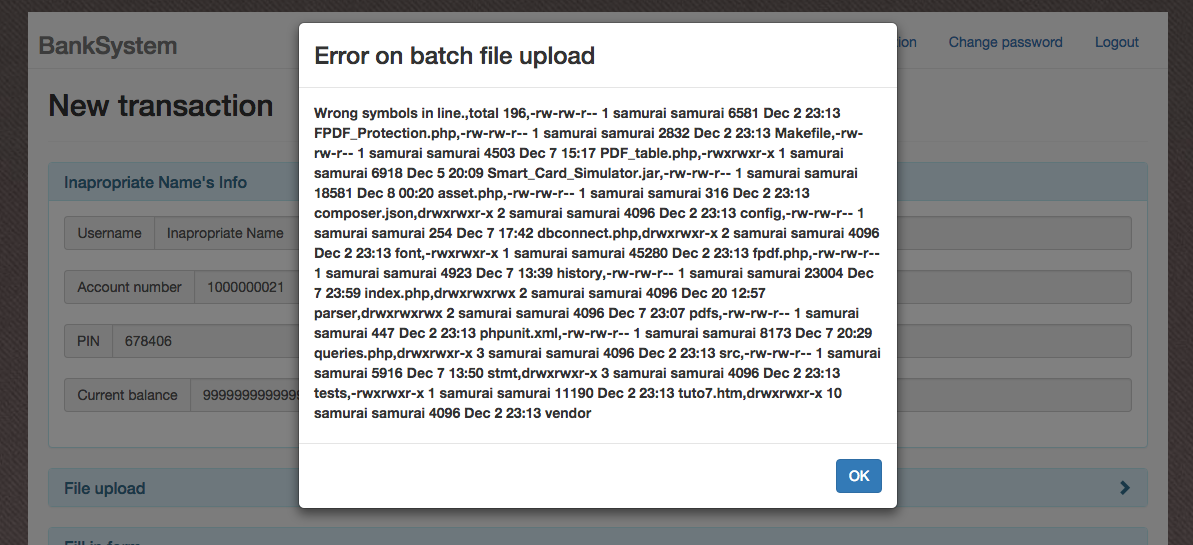
\includegraphics[width=\textwidth]{figures/bs_cmd_injection}
	\caption{Command injection example for the \bs{} application}
	\label{figure:bs_cmd_injection}
\end{figure}

\vulntitle{OTG-INPVAL-014}{Testing for Buffer overflow}
\vulntitle{OTG-INPVAL-014-2}{Testing for Stack overflow}
\vulntitle{OTG-INPVAL-014-3}{Testing for Heap overflow}
\vulntitle{OTG-INPVAL-014-4}{Testing for Format string}
\vulntitle{OTG-INPVAL-015}{Testing for incubated vulnerabilities}
\vultable{\bs}{%
	This has also been rectified as a part of the Phase III requirements. The code was inspected for input sensitization and Manual testing was done to confirm vulnerability was fixed.
}{%
\na
}{%
\na
}{%
\na
}{%
\na
}{%
\na
}
\vultable{\gnb}{%
	\same
}{%
\na
}{%
\na
}{%
\na
}{%
\na
}{%
\na
}
\vulntitle{OTG-INPVAL-016}{Testing for HTTP Splitting/Smuggling}
This vulnerability was not tested as we did not extend our testing to the Apache Web Server.

\clearpage
\section{Error Handling}
\simpleVulntitle{OTG-ERR-001}{Analysis of Error Codes}
\vultable{\bs}{%
	No vulnerabilities through Error Codes have been detected, although the one mentioned in \vulnref{OTG-IDENT-004} might be related because the error message is giving away that a valid mail address has been used. Please also refer to \vulnref{OTG-ERR-002} for error codes we found using the \texttt{api} functions, which also included slim stack traces.
}{%
	\na
}{%
	\na
}{%
	\na
}{%
	\na
}{%
	\secure
}
\vultable{\gnb}{%
	No Error Code vulnerabilities have been found in the \gnb{} application.
}{%
	\na
}{%
	\na
}{%
	\na
}{%
	\na
}{%
	\secure
}

\vulntitle{OTG-ERR-002}{Analysis of Stack Traces}
\vultable{\bs}{%
	The application uses REST calls between client and server, which can return stack traces whenever an error occurs in the Slim framework on the server. We managed to produce an example, as described in the discovery section below. These traces can only be seen in the REST response and not on the web interface.\newline
	We didn't manage to produce any other stack traces otherwise, neither on the SCS nor on the \bs{} web application. We discovered, however, that it is possible to produce buffer overflows on the C parser, although only locally and not through the web interface. For more information about this vulnerability, please refer to \vulnref{OTG-INPVAL-014}.
}{%
	We performed a REST request to the following link \texttt{https://[HOST]/api/uploadFile},using the Advanced REST Client extension for Chrome. We only used the following as a request parameter:
	\texttt{X-XSRF-TOKEN: a206758...08aa5cb}. Since the request would require more/different parameters, the application on server side generates an error, which is then returned to the client side as a REST response.
}{%
	The likelihood of an attacker testing the single REST APIs provided by the application is high.
}{%
	These errors are never displayed on the client side directly, but can nevertheless be seen using a REST client, providing an attacker with information about the source code on the server, along with details on where each error code is generated (refer to the example in the picture).
}{%
	The Slim framework produces stack traces automatically, hence the only way to avoid generating these is to check inside the PHP code if the expected variables are set. This can simply be done by calling the \texttt{isset(\$\_GET['paramName'])} function.
}{%
	\cvssBaseScorePretty{N}{L}{N}{N}{U}{L}{N}{N}
}
\vultable{\gnb}{%
	We did not manage to produce any stack traces, neither on the SCS application nor on the \gnb{} web application itself.
}{%
	We intensively tested the application in order to produce stack traces, with no results. The testing for this purpose was done manually.
}{%
	\na
}{%
	\na
}{%
	\na
}{%
	\secure
}

\begin{figure}[h!tbp]
	\centering
	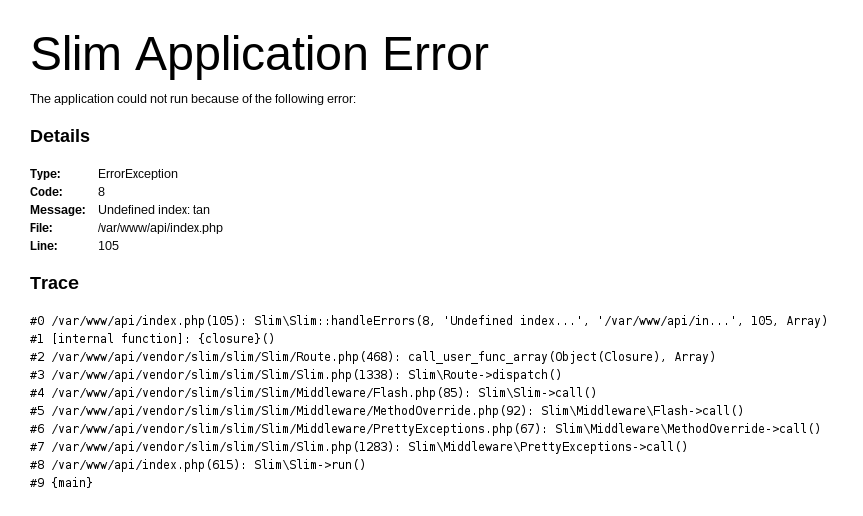
\includegraphics[width=\textwidth]{figures/Slim_StackTrace}
	\caption{Example of a Slim application error}
	\label{figure:Slim_StackTrace}
\end{figure}


\clearpage
\section{Cryptography}
\simpleVulntitle{OTG-CRYPST-001}{Testing for Weak SSL/TSL Ciphers, Insufficient Transport Layer Protection}
\vultable{\bs}{%
	This was tested using a script listed on the OWASP website \href{https://testssl.sh/}{TestSSL}, this ran a list of tests on SSL, (see \autoref{figure:bs_ssl_cipher} and \autoref{figure:bs_ssl_vuln}).	
}{%
	This application reported the following main vulnerabilities:
	\begin{itemize}
		\setlength\itemsep{0pt}  
		\item Vulnerable to \href{https://web.nvd.nist.gov/view/vuln/detail?vulnId=CVE-2014-0160 }{Heartbleed}
		\item Vulnerable to \href{https://web.nvd.nist.gov/view/vuln/detail?vulnId=CVE-2014-0224 }{CCS}
		\item Vulnerable to \href{https://web.nvd.nist.gov/view/vuln/detail?vulnId=CVE-2014-3566 }{POODLE}
		\item Vulnerable to \href{https://web.nvd.nist.gov/view/vuln/detail?vulnId=CVE-2013-2566 }{RC4 \#1}
		\item Vulnerable to \href{https://web.nvd.nist.gov/view/vuln/detail?vulnId=CVE-2015-2808 }{RC4 \#2}
	\end{itemize}
}{%
	\begin{description}
		\item[Heartbleed] Heartbleed while talked about it often when mentioning SSL, still requires some technical knowledge, which is readily available online with instructions and hence the likelihood is high.
		\item[CCS]
		In order to exploit CCS it requires the attacker to intercept and alter network traffic in real time. This reduces the risk and likelihood of this vulnerability.
		\item[POODLE]
		POODLE exploit tools are already in development, however this attack only works with SSL 3.0 which is being phased out at the moment.
		\item[RC4]
		The RC4 algorithm has many single-byte biases, making it susceptible to statistical attacks, which require some technical knowledge and hence the likelihood is not high.
	\end{description}
}{%
	With the exception on Heartbleed which allows the attackers to read server memory, the rest of the attacks impact lies in eavesdropping on encrypted packets.
}{%
	\begin{itemize}  
		\item Install system security updates especially Apache and SSL
		\item Disable SSLv3, Medium grade encryption, Triple DES and other weak ciphers
	\end{itemize}
}{%
	\cvssBaseScorePretty{N}{H}{N}{N}{C}{H}{N}{N}
}
	\begin{figure}[h!tbp]
		\centering
		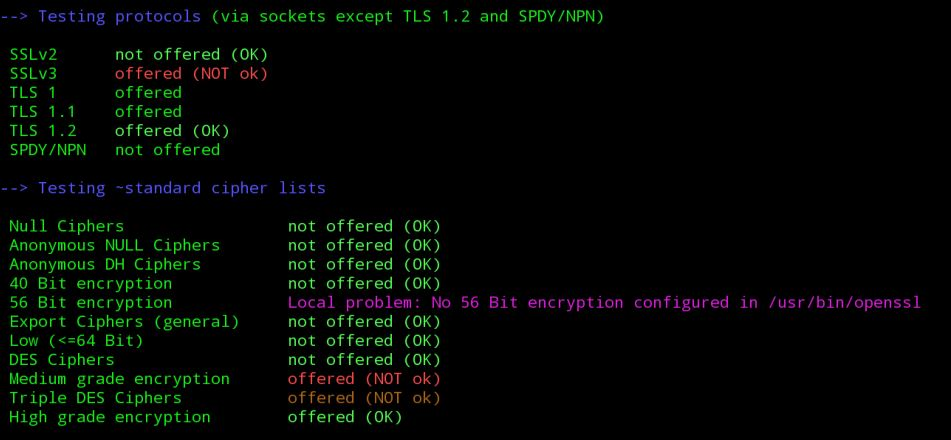
\includegraphics[width=\textwidth]{figures/t07_ssl_cipher.png}
		\caption{SSL Ciphers used by \bs application}
		\label{figure:bs_ssl_cipher}
	\end{figure}
	\begin{figure}[h!tbp]
		\centering
		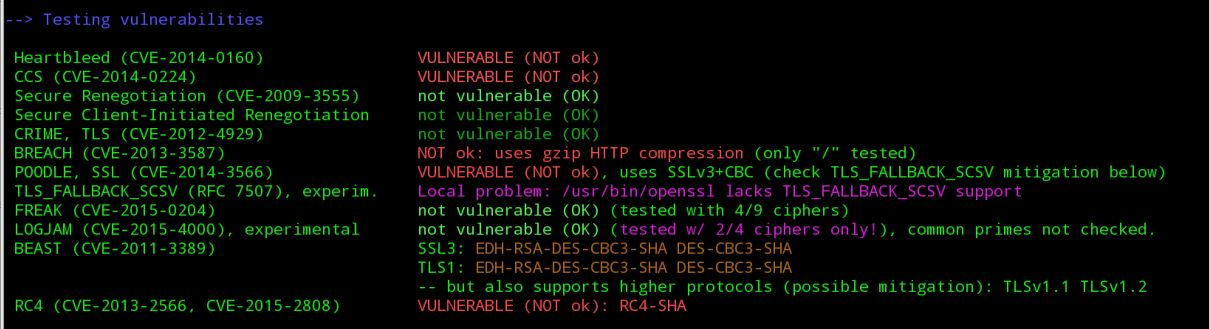
\includegraphics[width=\textwidth]{figures/t07_ssl_vuln.png}
		\caption{SSL Vulnerabilities used by \bs application}
		\label{figure:bs_ssl_vuln}
	\end{figure}

\vultable{\gnb}{%
	\same, (see \autoref{figure:gnb_ssl_cipher} and \autoref{figure:gnb_ssl_vuln}).	
}{%
	This application reported the following main vulnerabilities:
	\begin{itemize}
		\setlength\itemsep{0pt}  
		\item Vulnerable to \href{https://web.nvd.nist.gov/view/vuln/detail?vulnId=CVE-2014-3566 }{POODLE}
		\item Vulnerable to \href{https://web.nvd.nist.gov/view/vuln/detail?vulnId=CVE-2013-2566 }{RC4 \#1}
		\item Vulnerable to \href{https://web.nvd.nist.gov/view/vuln/detail?vulnId=CVE-2015-2808 }{RC4 \#2}
	\end{itemize}
}{%
	\begin{description}
		\item[POODLE]
		POODLE exploit tools are already in development, however this attack only works with SSL 3.0 which is being phased out at the moment.
		\item[RC4]
		The RC4 algorithm has many single-byte biases, making it susceptible to statistical attacks, which require some technical knowledge and hence the likelihood is not high.
	\end{description}
}{%
	Both attacks lead to eavesdropping on encrypted packets.
}{%
	To fix the vulnerabilities above the following is recommended:
	\begin{itemize}
		\item Disable SSLv3, Medium grade encryption, Triple DES and other weak ciphers
	\end{itemize}
}{%
	\cvssBaseScorePretty{N}{H}{N}{R}{U}{L}{N}{N}
}
	\begin{figure}[h!tbp]
		\centering
		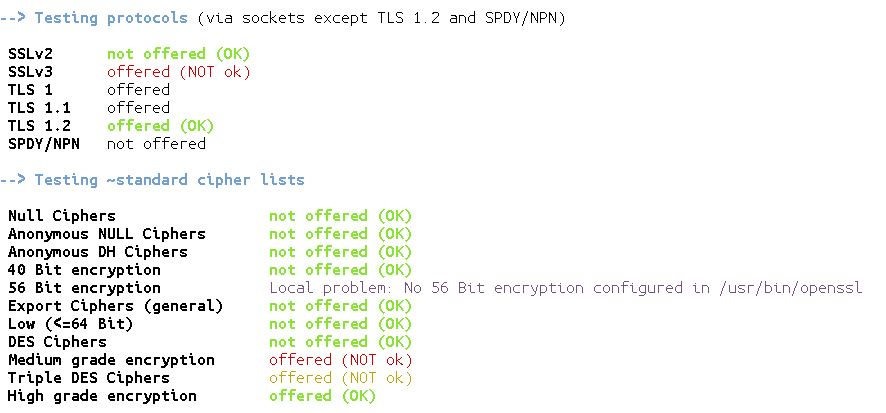
\includegraphics[width=\textwidth]{figures/t12_ssl_cipher.png}
		\caption{SSL Ciphers used by \gnb application}
		\label{figure:gnb_ssl_cipher}
	\end{figure}
	\begin{figure}[h!tbp]
		\centering
		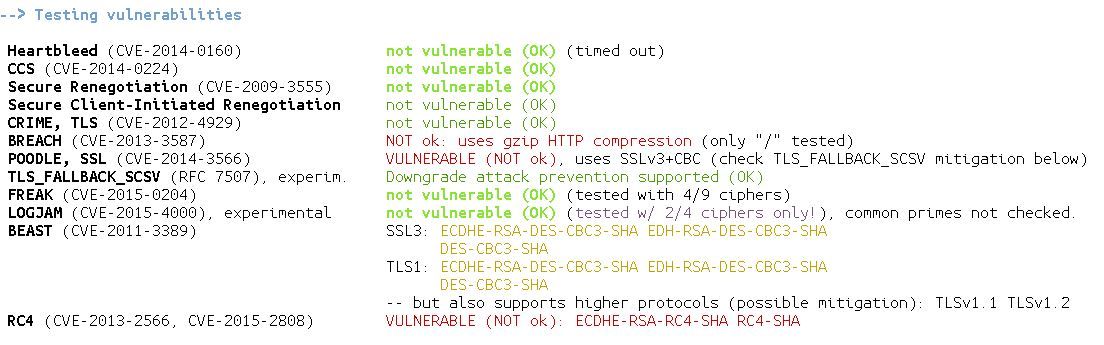
\includegraphics[width=\textwidth]{figures/t12_ssl_vuln.png}
		\caption{SSL Vulnerabilities used by \gnb application}
		\label{figure:gnb_ssl_vuln}
	\end{figure}

\vulntitle{OTG-CRYPST-002}{Testing for Padding Oracle}
\vultable{\bs}{%
	\notImp
}{%
	\na
}{%
	\na
}{%
	\na
}{%
	\na
}{%
	\na
}
\vultable{\gnb}{%
	\notImp
}{%
	\na
}{%
	\na
}{%
	\na
}{%
	\na
}{%
	\secure
}

\vulntitle{OTG-CRYPST-003}{Testing for Sensitive information sent via unencrypted channels}
\vultable{\bs}{%
	All request to the site are done over an encrypted HTTPS connection. No unencrypted messages were observed.
}{%
	After capturing the traffic of normal application use with wireshark, it was verified that all requests made were encrypted.
}{%
	\na
}{%
	\na
}{%
	\na
}{%
	\secure
}
\vultable{\gnb}{%
	All request to the site are done over an encrypted HTTPS connection. No unencrypted messages were observed.
}{%
	After capturing the traffic of normal application use with wireshark, it was verified that all requests made were encrypted.
}{%
	\na
}{%
	\na
}{%
	\na
}{%
	\secure
}

\clearpage
\section{Business Logic Testing}
\simpleVulntitle{OTG-BUSLOGIC-001}{Test Business Logic Data Validation}
\vultable{\bs}{%
	While testing the whole application, we discovered that only valid data is accepted, not allowing to exploit the application in any way by inserting invalid data. \newline
}{%
	We statically analyzed the PHP source code using RIPS, RATS and later on went through the code manually, in order to find additional vulnerabilities not detected by the previously mentioned tools. RIPS and RATS also produced some false positives, like the \texttt{\$tan} field inside the multiple transaction callback function (/api/index.php line 105): in this example the variable was marked as a vulnerability, although the data is validated by the application at a later moment in time.
}{%
	\na
}{%
	\na
}{%
	\na
}{%
	\secure
}
\vultable{\gnb}{%
	While testing the whole application, we discovered that only valid data is accepted, not allowing to exploit the application in any way by inserting invalid data. \newline
	As described in \ref{chapter:reverse_engineering} (SCS analysis) however, after a specific point in time, user input will no longer be validated correctly, because of a timestamp overflow bug in the Java code. This cannot be considered a vulnerability, but will pose a problem for clients in the future (in 22 years time).
}{%
	We statically analyzed the PHP source code using RIPS, RATS and later on went through the code manually, in order to find additional vulnerabilities not detected by the previously mentioned tools. Also, RIPS and RATS mainly produced false positives.
}{%
	\na
}{%
	\na
}{%
	\na
}{%
	\secure
}

\vulntitle{OTG-BUSLOGIC-002}{Test Ability to Forge Requests}
\vultable{\bs}{%
	No vulnerabilities in this area were found for the \bs{} application.
}{%
	\na
}{%
	\na
}{%
	\na
}{%
	\na
}{%
	\secure
}
\vultable{\gnb}{%
	No vulnerabilities in this area were found for the \gnb{} application.
}{%
	\na
}{%
	\na
}{%
	\na
}{%
	\na
}{%
	\na
}

\vulntitle{OTG-BUSLOGIC-003}{Test Integrity Checks}
\vultable{\bs}{%
	\notImp
}{%
	\na
}{%
	\na
}{%
	\na
}{%
	\na
}{%
	\na
}
\vultable{\gnb}{%
	\notImp
}{%
	\na
}{%
	\na
}{%
	\na
}{%
	\na
}{%
	\na
}

\vulntitle{OTG-BUSLOGIC-004}{Test for Process Timing}
\vultable{\bs}{%
	We observed that the \bs{} application has a process timing vulnerability in the login function. 
	The login page would reply within 50ms if the mail address was valid and within around 20ms if the mail address was not valid.
}{%
	We observed that by looking at the source code for the login (see \texttt{api/index.php} lines 168-304) and confirming our observations by black box testing.
}{%
	It is quite likely that this vulnerability is used for finding valid mail addresses, although in this particular case another vulnerability (see \vulnref{OTG-IDENT-004}) is much easier to exploit for this attack.
}{%
	\na
}{%
	\na
}{%
	\cvssBaseScorePretty{N}{L}{N}{N}{U}{L}{N}{N}
}
\vultable{\gnb}{%
	No Process Timing vulnerability was found in the \gnb{} application.
}{%
	\na
}{%
	\na
}{%
	\na
}{%
	\na
}{%
	\secure
}

\vulntitle{OTG-BUSLOGIC-005}{Test Number of Times a Function Can be Used Limits}
\vultable{\bs}{%
	While reviewing the project documentation and testing the single functionalities we did not find any possible application misuse/abuse cases that would allow a user to execute a function more than the allowable number of times.
}{%
	We performed manual tests on all application features.
}{%
	\na
}{%
	\na
}{%
	\na
}{%
	\secure
}
\vultable{\gnb}{%
	The same observations made for the \bs{} application hold.
}{%
	\same
}{%
	\na
}{%
	\na
}{%
	\na
}{%
	\secure
}

\vulntitle{OTG-BUSLOGIC-006}{Testing for the Circumvention of Work Flows}
\vultable{\bs}{%
	The follow cases were tested based on the report submittid from team 7 in Phase II
	\begin{itemize}
		\item Customer ability to access employee portal.
		\item Customer approving his own transaction.							
		\item Customer accessing account before account being approved.
		\item Customer bypassing approval for large transaction.	
	\end{itemize}
	
	By inspecting the code, proper checks have been put in place that disallow circumvention in the above cases.
	
}{%
\na
}{%
\na
}{%
\na
}{%
\na
}{%
\secure
}
\vultable{\gnb}{%
}{%
Vulnerabilities in this seciton were rectified as part of the requirements for phase III.
}{%
\na
}{%
\na
}{%
\na
}{%
\secure
}

\vulntitle{OTG-BUSLOGIC-007}{Test Defenses Against Application Mis-use}
\vultable{\bs}{%
	No mechanisms to prevent against application mis-use are in place except the lockout-functionality (see \vulnref{OTG-AUTHN-003}). No critical functionalities are disabled and no logs are kept.
}{%
	These observations were made after reading the source code and testing the accuracy of the observations with some manual testing.
}{%
	The likelihood of exploiting this vulnerability is high because all standard fuzzying tools are able to exploit this vulnerability, even making it possible for so-called "script-kiddies" to try their luck.
}{%
	Given the other observations about the \bs{} application the impact of this vulnerability is not really high as this will probably not lead to a security breach.
}{%
	We recommend to implement a simple way to detect malicious requests and prevent further requests for some time after a certain treshold is reached.
}{%
	\cvssBaseScorePretty{N}{L}{N}{N}{U}{L}{L}{L}
}
\vultable{\gnb}{%
	\same
}{%
	\same
}{%
	\same
}{%
	\same
}{%
	\same
}{%
	\cvssBaseScorePretty{N}{L}{N}{N}{U}{L}{L}{L}
}

\vulntitle{OTG-BUSLOGIC-008}{Test Upload of Unexpected File Types}
\vultable{\bs}{%
	Only files with the MIME-type \texttt{text/plain} are allowed. The file is
	renamed on the server side to a random string with a \texttt{.txt} file
	extension. The file is deleted directly after processing.
}{%
	We obtained the allowed file types by inspecting the code and manually
	verifying the results by testing the file upload afterwards.
}{%
	\na
}{%
	\na
}{%
	\na
}{%
	\secure
}
\vultable{\gnb}{%
	The files are renamed on upload to the sessionid without extention. The c
	parser ignores files with only invalid transaction details afterwards.
	The file is deleted directly after processing.
}{%
	\same
}{%
	\na
}{%
	\na
}{%
	Additionally filter for mime type and/or file extention before accepting
	the file upload.
}{%
	\secure
}

\vulntitle{OTG-BUSLOGIC-009}{Test Upload of Malicious Files}
\vultable{\bs}{%
	We discovered that it is possible to upload malicious files using the batch transaction functionality: these files won't be recognised by the target system as malwares, but these files cannot bring any harm to the application. This is because the uploaded files are automatically renamed and removed from the system after executing the C parser. Since the C parser reads the the uploaded files as simple text files, nothing bad can happen.
}{%
	We tried uploading test malwares found in the Internet, as well as custom PHP/bash scripts. Since the application only allows text extensions, so we had to rename them first, before uploading them. All files were accepted by the server, but the transactions simply failed as a result.
}{%
	\na
}{%
	\na
}{%
	\na
}{%
	\secure
}
\vultable{\gnb}{%
	The same observations made for the \bs{} application hold.
}{%
	\same
}{%
	\na
}{%
	\na
}{%
	\na
}{%
	\secure
}

\clearpage
\section{Client Side Testing}
\simpleVulntitle{OTG-CLIENT-001}{Testing for DOM based Cross Site Scripting}
\vultable{\bs}{%
	see \vulnref{OTG-INPVAL-001}
}{%
\na
}{%
\na
}{%
\na
}{%
\na
}{%
\secure
}
\vultable{\gnb}{%
	\same
}{%
\na
}{%
\na
}{%
\na
}{%
\na
}{%
\secure
}
\vulntitle{OTG-CLIENT-002}{Testing for JavaScript Execution}
Please refer to \vulnref{OTG-INPVAL-001} and \vulnref{OTG-INPVAL-002}.

\vulntitle{OTG-CLIENT-003}{Testing for HTML Injection}
\vultable{\bs}{%
	We discovered that it is not possible to perform HTML injection attacks on the \bs{} application, although some user input isn't properly sanitized by the server (e.g. Description field in a transaction). This does not pose a threat, however, since the application is based on the AngularJS framework, which sanitizes the user input automatically on the client (see image below). Refer to \vulnref{OTG-INPVAL-002} for more details.
}{%
	We manually analyzed the client-side code of the \bs{} application, looking for \texttt{.innerHTML} and \texttt{document.write} potential vulnerabilities, not finding any.
}{%
	\na
}{%
	\na
}{%
	\na
}{%
	\secure
}
\vultable{\gnb}{%
	We didn't find any HTML injection vulnerability, since all user input is sanitized by the server for each GET/POST request.
}{%
	We manually analyzed the client-side and server-side code, looking for potential HTML injection vulnerabilities.
}{%
	\na
}{%
	\na
}{%
	\na
}{%
	\secure
}

\begin{figure}[h!tbp]
	\centering
	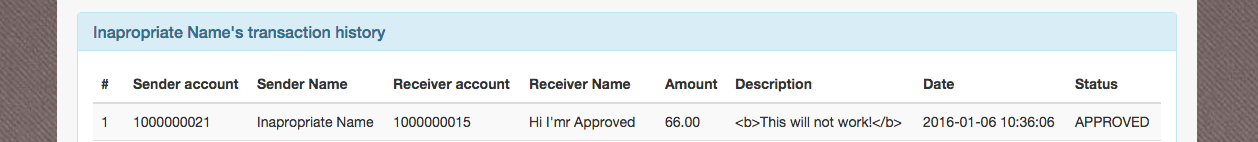
\includegraphics[width=\textwidth]{figures/bs_html_injection}
	\caption{HTML injection attempt inside a description field}
	\label{figure:bs_html_injection}
\end{figure}


\vulntitle{OTG-CLIENT-004}{Testing for Client Side URL Redirect}
\vultable{\bs}{%
	While analyzing the Javascript code, we did not find any URL redirection vulnerabilities. The Bank System application exploits the AngularJS framework and moves between pages using static strings, never using any unsanitized user input as a target URL. The backend also never performs redirection using a GET/POST parameter as the target URL.
}{%
	We accurately inspected all the client-side code and the PHP server-side code where URL redirections take place.
}{%
	\na
}{%
	\na
}{%
	\na
}{%
	\secure
}
\vultable{\gnb}{%
	While testing the Javascript code, we did not find any URL redirection vulnerabilities. Whenever a page is redirected using the \texttt{window.location} object, a static string is directly assigned to it, never using any unsanitized user input as a variable. The backend also never performs redirection using a GET/POST parameter as the target URL.
}{%
	We accurately inspected all the client-side code and the PHP server-side code where URL redirections take place. In the latter case, the \gnb{} application performs redirections only exploiting the \texttt{resource\_mappings.php} file and not redirecting directly to a URL contained in a parameter.
}{%
	\na
}{%
	\na
}{%
	\na
}{%
	\secure
}

\vulntitle{OTG-CLIENT-005}{Testing for CSS Injection}
\vultable{\bs}{%
	This vulnerability is not available as no code is injectable in the CSS files or styles in HTML or PHP files.
}{%
\na
}{%
\na
}{%
\na
}{%
\na
}{%
\secure
}
\vultable{\gnb}{%
	\same
}{%
\na
}{%
\na
}{%
\na
}{%
\na
}{%
\secure
}
\vulntitle{OTG-CLIENT-006}{Testing for Client Side Resource Manipulation}
\vultable{\bs}{%
	No Client Side Resource Manipulation vulnerability was found in the \bs{} application.
}{%
	This was observed by manually looking through the source code as none of the used tools covered this area.
}{%
	\na
}{%
	\na
}{%
	\na
}{%
	\secure
}
\vultable{\gnb}{%
	No Client Side Resource Manipulation vulnerability was found in the \gnb{} application.
}{%
	\same
}{%
	\same
}{%
	\same
}{%
	\same
}{%
	\secure
}

\vulntitle{OTG-CLIENT-007}{Test Cross Origin Resource Sharing}
\vultable{\bs}{%
	\notImp
}{%
	\na
}{%
	\na
}{%
	\na
}{%
	\na
}{%
	\na
}
\vultable{\gnb}{%
	\notImp
}{%
	\na
}{%
	\na
}{%
	\na
}{%
	\na
}{%
	\na
}

\vulntitle{OTG-CLIENT-008}{Testing for Cross Site Flashing}
\vultable{\bs}{%
	This vulnerability doesn't apply for the tested applications, since Flash is not used.
}{%
	\na
}{%
	\na
}{%
	\na
}{%
	\na
}{%
	\na
}
\vultable{\gnb}{%
	This vulnerability doesn't apply for the tested applications, since Flash is not used.
}{%
	\na
}{%
	\na
}{%
	\na
}{%
	\na
}{%
	\na
}

\vulntitle{OTG-CLIENT-009}{Testing for Clickjacking}
\vultable{\bs}{%
	This vulnerability was meant to be fixed as part of the Phase III requirements.
}{%
The \bs Application has no protection (X-Frame-Options header) against Click-Jacking attacks. This vulnerability was found using w3af.
}{%
This is a relatively easy attack, not much technical knowledge is needed.
}{%
Depending on the skill of the attacker has, but can potentially take control of certain aspects of the victims computer such as camera and microphone.
}{%
\begin{itemize}
	\item Sending the proper X-Frame-Options HTTP response headers that instruct the browser to not allow framing from other domains
	\item Employing defensive code in the UI to ensure that the current frame is the most top level window
\end{itemize}
}{%
\cvssBaseScorePretty{N}{H}{N}{R}{C}{L}{L}{N}
}
\vultable{\gnb}{%
	This vulnerability was fixed as part of the phase 3 requirements.
}{%
\na
}{%
\na
}{%
\na
}{%
\na
}{%
\secure
}

\vulntitle{OTG-CLIENT-010}{Testing WebSockets}
\vultable{\bs}{%
	\notImp
}{%
	\na
}{%
	\na
}{%
	\na
}{%
	\na
}{%
	\na
}
\vultable{\gnb}{%
	\notImp
}{%
	\na
}{%
	\na
}{%
	\na
}{%
	\na
}{%
	\na
}

\vulntitle{OTG-CLIENT-011}{Test Web Messaging}
\vultable{\bs}{%
	\notImp
}{%
	\na
}{%
	\na
}{%
	\na
}{%
	\na
}{%
	\na
}
\vultable{\gnb}{%
	\notImp
}{%
	\na
}{%
	\na
}{%
	\na
}{%
	\na
}{%
	\na
}

\vulntitle{OTG-CLIENT-012}{Test Local Storage}
\vultable{\bs}{%
	\notImp
}{%
	\na
}{%
	\na
}{%
	\na
}{%
	\na
}{%
	\na
}
\vultable{\gnb}{%
	\notImp
}{%
	\na
}{%
	\na
}{%
	\na
}{%
	\na
}{%
	\na
}
